\documentclass[11pt]{article}
\usepackage[T1]{fontenc}
\usepackage[margin=0.88in]{geometry}
\usepackage{amsmath,amssymb,amsthm}
\usepackage{graphicx}
\usepackage{microtype}
\usepackage{xcolor}
\usepackage[colorlinks=true,linkcolor=blue!55!black,urlcolor=blue!65!black]{hyperref}

\newtheorem{theorem}{Theorem}
\newtheorem{lemma}{Lemma}
\newcommand{\C}{\mathcal C}
\newcommand{\F}{\mathcal F}
\newcommand{\R}{\mathbb R}
\newcommand{\rhoo}{\varrho^{*}}

\title{Nonlinear recovery relative to Kolmogorov width is\\
equivalent to one-sided discretization}
\author{Candidate strong partial result for arXiv:2402.00848}
\date{12 August 2026}

\begin{document}
\maketitle

\begin{center}
\fbox{\begin{minipage}{0.92\textwidth}
\textbf{Status: strong partial result, likely valid.}
For every finite $p$, dimension $N$, and sample budget $m$, the worst-case
constant in nonlinear recovery relative to the $N$th $L_\infty$ Kolmogorov
width is within explicit affine constants of the worst-case one-sided
$L_p$ discretization constant.  Thus Open Problems 3.1 and 5.1 of the source
are quantitatively equivalent.  The common optimal growth rate and the linear
recovery problem remain open.
\end{minipage}}
\end{center}

\section{Source questions and definitions}

The source is I.~Limonova, Yu.~Malykhin, and V.~Temlyakov,
\emph{One-sided discretization inequalities and sampling recovery},
arXiv:2402.00848.  Let $\Omega$ be compact, let $\mu$ be a probability
measure, and let $X\subset\C(\Omega)$ be $N$-dimensional.  For sampling points
$\xi=(\xi^1,\ldots,\xi^m)$, put
\[
 D(X,\xi):=\sup_{0\ne x\in X}
 \frac{\|x\|_{L_p(\mu)}}{\max_j|x(\xi^j)|},
\]
with value $+\infty$ when the sampling map is not injective, and put
$D_m(X)=\inf_\xi D(X,\xi)$.  The universal constant is
\[
 D_{m,p}(N):=\sup_{(\Omega,\mu),\ \dim X=N}D_m(X).
\]

For a compact class $\F\subset\C(\Omega)$, let $d_N(\F,L_\infty)$ be its
$N$th Kolmogorov width.  The nonlinear sampling error $\rhoo_m(\F,L_p)$ is
the infimum, over $m$ sampling points and all reconstruction maps whose range
lies in an at-most-$m$-dimensional linear subspace, of the worst $L_p$ error.
Define
\[
 R^*_{m,p}(N):=sup_{(\Omega,\mu),\ \F}
 \frac{\rhoo_m(\F,L_p)}{d_N(\F,L_\infty)},
\]
where the supremum ranges over compact classes with nonzero width.

Open Problem 3.1 asks for the growth of $m$ making $D_{m,p}(N)$ bounded by a
constant depending only on $p$, for $2<p<\infty$.  Open Problem 5.1 asks for
the growth making $R^*_{m,p}(N)$ bounded.  Open Problem 5.2 asks the analogous
question for linear reconstruction.

\begin{figure}[p]
\centering
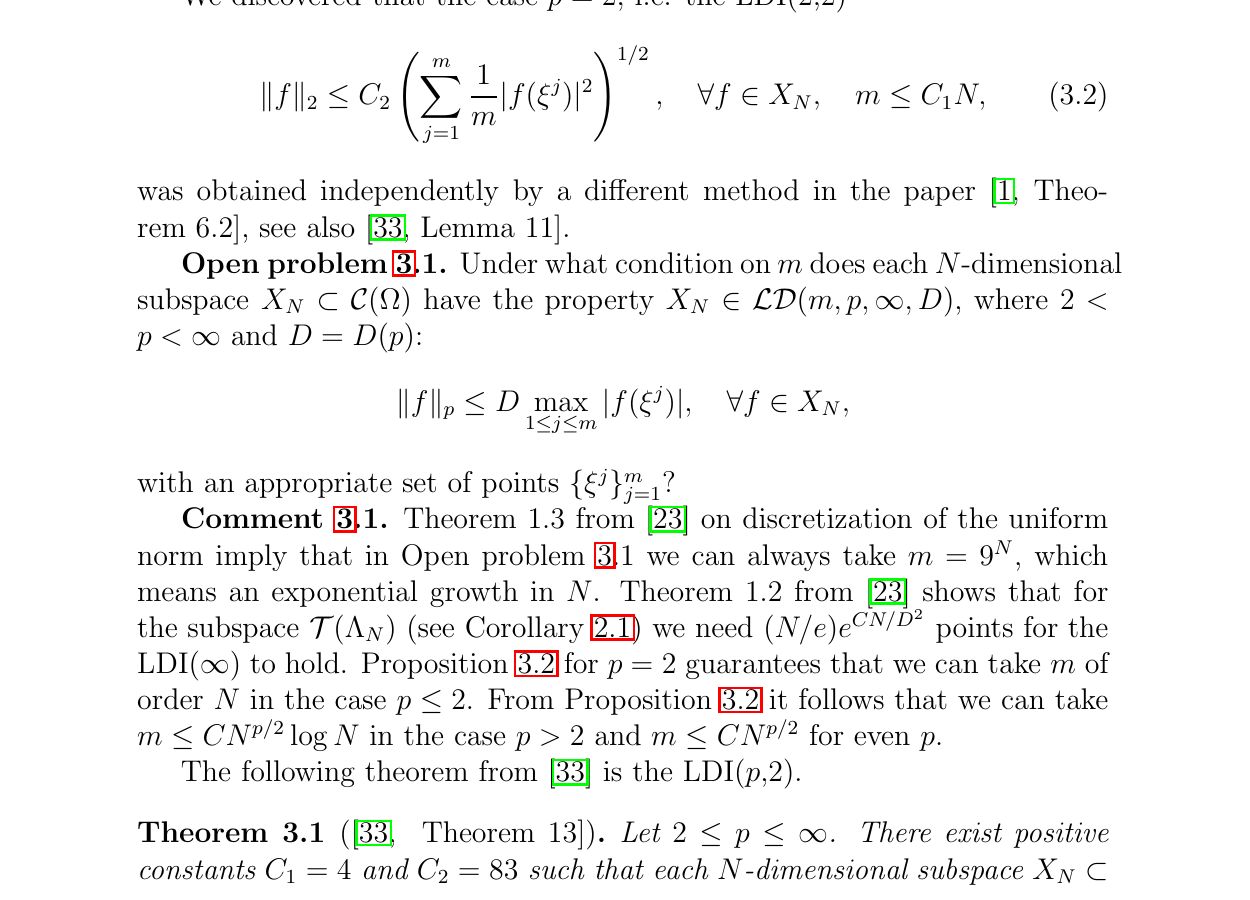
\includegraphics[width=0.96\textwidth]{figures/open_problem_3_1_crop.png}
\caption{Open Problem 3.1 and the source's known bounds, official arXiv PDF,
page 14.}
\end{figure}

\begin{figure}[p]
\centering
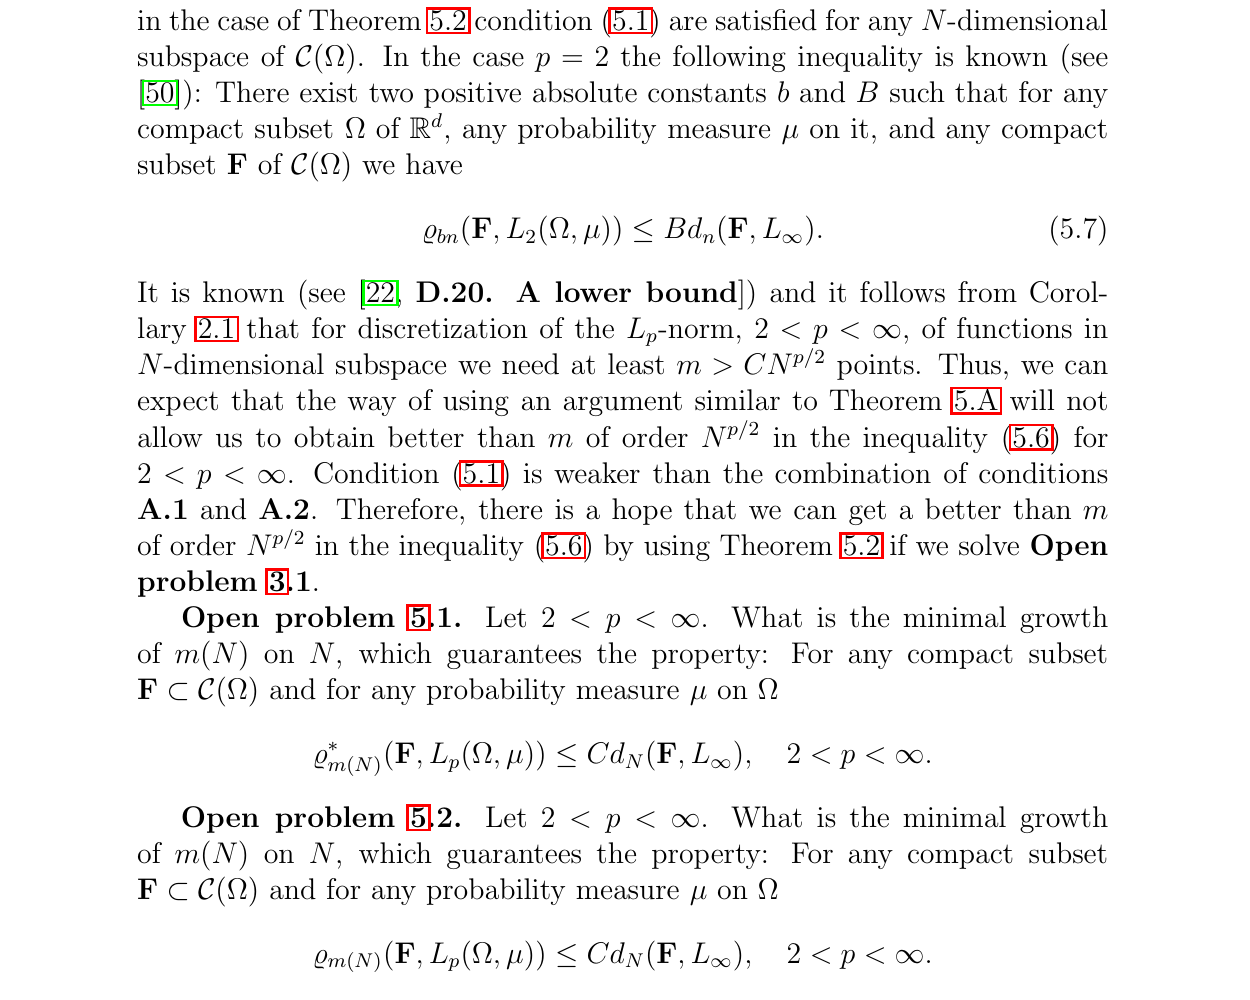
\includegraphics[width=0.96\textwidth]{figures/open_problems_5_1_5_2_crop.png}
\caption{Open Problems 5.1 and 5.2, official arXiv PDF, page 22.}
\end{figure}

\clearpage
\section{Proof Intuition}

The easy direction is the source's recovery argument: a sample set which
norms every vector of an approximating subspace lets one convert small sampled
residual into small $L_p$ residual.

For the reverse direction, start with a subspace that no $m$ samples norm
well.  Its $L_p$ unit ball by itself has zero $N$th width, so it cannot test a
width inequality.  Thicken that ball by a compact family of uniformly small
functions.  The family is chosen canonically: pointwise clip each unit-ball
element to the disk of radius $\varepsilon$.  Given any proposed sample set,
choose a unit vector whose sampled values are at most $\varepsilon$ and
subtract its clip.  This erases every observation but leaves $L_p$ norm at
least $1-\varepsilon$.  The opposite function has the same zero data, so no
algorithm can approximate both.  Meanwhile the entire thickened class stays
within $\varepsilon$ in $L_\infty$ of the original $N$-space.

\section{Quantitative equivalence}

For $\varepsilon>0$, let $c_\varepsilon:\mathbb C\to\mathbb C$ be radial
clipping onto the closed disk of radius $\varepsilon$:
\[
 c_\varepsilon(z)=
 \begin{cases}
 z,&|z|\le\varepsilon,\\
 \varepsilon z/|z|,&|z|>\varepsilon.
 \end{cases}
\]
For real scalars this is ordinary clipping to
$[-\varepsilon,\varepsilon]$.  It acts pointwise on continuous functions.

\begin{theorem}\label{thm:main}
For every $1\le p<\infty$ and all positive integers $m,N$,
\[
 \boxed{\quad D_{m,p}(N)-1\ \le\ R^*_{m,p}(N)\
 \le\ 2D_{m,p}(N)+1.\quad}
\]
In particular, a function $m=m(N)$ gives a dimension-free one-sided
discretization constant if and only if it gives a dimension-free nonlinear
recovery-to-width constant.
\end{theorem}

\begin{proof}
We first prove the upper bound, including the short source mechanism.  Fix a
compact class $\F$ and $\eta>0$, and choose an $N$-dimensional space $X$ such
that
\[
 \sup_{f\in\F}d(f,X)_\infty
 \le (1+\eta)d_N(\F,L_\infty).
\]
Choose $m$ samples with $D(X,\xi)\le D_{m,p}(N)+\eta$.  For each $f$, let
$u\in X$ minimize the sampled $\ell_\infty$ residual, and choose $h\in X$
arbitrarily close to a best uniform approximant.  Minimality gives
\[
 \max_j|(h-u)(\xi^j)|
 \le 2\|f-h\|_\infty.
\]
Consequently,
\[
 \|f-u\|_p
 \le \|f-h\|_p+\|h-u\|_p
 \le \bigl(1+2D(X,\xi)\bigr)\|f-h\|_\infty.
\]
Letting the approximation errors and $\eta$ tend to zero yields
$R^*_{m,p}(N)\le2D_{m,p}(N)+1$.

For the converse, fix $X$ and write $D=D_m(X)$.  The claim is trivial when
$D\le1$, so assume $1<D<\infty$ and put $\varepsilon=D^{-1}$.  Let
\[
 U=\{x\in X:\|x\|_p\le1\},\qquad
 H_\varepsilon=\{-c_\varepsilon\circ x:x\in U\},\qquad
 \F_X=U+H_\varepsilon.
\]
The set $U$ is compact in the uniform norm because $X$ is finite-dimensional.
Pointwise clipping is continuous in that norm, so $H_\varepsilon$ and
$\F_X$ are compact.  Moreover, every $x+h\in\F_X$ is within
$\|h\|_\infty\le\varepsilon$ of $X$, whence
\[
 d_N(\F_X,L_\infty)\le\varepsilon.
\]

Now fix \emph{arbitrary} $m$ sampling points $\xi$.  Since
$D(X,\xi)\ge D$, compactness of the $L_p$ unit sphere gives an $x\in X$ with
\[
 \|x\|_p=1,
 \qquad \max_j|x(\xi^j)|\le D^{-1}=\varepsilon.
\]
(If the sampling map has a kernel, take a unit vector in it.)  Hence
\[
 f=x-c_\varepsilon\circ x\in\F_X,
 \qquad f(\xi^j)=0\quad(1\le j\le m),
\]
and, because $\mu$ is a probability measure,
\[
 \|f\|_p\ge1-\|c_\varepsilon\circ x\|_p\ge1-\varepsilon.
\]
The clipping map is odd, so $-f\in\F_X$ as well.  Both functions produce the
same zero sample vector.  If an arbitrary reconstruction map returns $g$ on
that vector, the triangle inequality gives
\[
 \max\{\|f-g\|_p,\|-f-g\|_p\}\ge\|f\|_p\ge1-\varepsilon.
\]
This holds for every sample set and every reconstruction map, even without a
range restriction.  Therefore
\[
 \frac{\rhoo_m(\F_X,L_p)}{d_N(\F_X,L_\infty)}
 \ge \frac{1-\varepsilon}{\varepsilon}=D-1.
\]
Taking the supremum over $X$ proves the lower bound.  If $D_m(X)=\infty$,
the same construction with arbitrary $\varepsilon>0$ gives an unbounded
ratio, so the extended-real statement also follows.
\end{proof}

\section{Consequences, verification, and limitations}

The theorem turns the source's sufficient implication into an if-and-only-if
statement with constants:
\[
 D_{m,p}(N)\le R^*_{m,p}(N)+1,
 \qquad R^*_{m,p}(N)\le2D_{m,p}(N)+1.
\]
Thus Open Problem 5.1 cannot have a better universal sampling growth than Open
Problem 3.1.  Any lower bound, logarithmic obstruction, or optimal theorem for
one problem transfers immediately to the other.

The obstruction applies to every recovery rule, so if $R_{m,p}(N)$ denotes
the linear-recovery analogue, then
\[
 D_{m,p}(N)-1\le R^*_{m,p}(N)\le R_{m,p}(N).
\]
The missing reverse bound for $R_{m,p}(N)$ is substantive: the sampled
$\ell_\infty$ best-approximation map used above is nonlinear, while a bounded
linear inverse/extension can incur a dimension-dependent projection constant.
Hence the proof does not solve Open Problem 5.2.

\paragraph{Verification.}
The script \texttt{code/verify\_finite\_obstruction.py} exhausts all 120
two-point sample sets for twenty rotations of a sixteen-point circular model.
It computes the sampling-polytope vertices, constructs the pointwise
cancellation, and checks the zero data, uniform perturbation bound, $L_p$
lower bound, and ratio inequality.  It ends with
\texttt{ALL FINITE OBSTRUCTION CHECKS PASSED}.  This is a sanity check; the
proof above is exact and non-computational.

\paragraph{Upgrade attempts.}
Eight focused routes were pursued: even-moment tensorization, Lewis-position
sparsification, rare-spike random sampling, VC hitting sets, symmetric lower
examples, sparse-spike constructions, linear extension, and later-literature
search.  They did not close the known $N^{p/2}$ versus
$N^{p/2}\log N$ gap for non-even $p$ or produce a linear-recovery upper bound.
Details are in the associated attempt note.

\paragraph{Novelty audit.}
The source PDF and TeX were inspected.  Bounded arXiv searches through
12 August 2026 used the exact title, authors, open-problem language,
``one-sided discretization'', ``sampling recovery'', and the $N^{p/2}$ scale.
They found the source, standard norm-discretization papers, and the 2026
Dai--Temlyakov survey, but no converse via a compact thickened unit ball and no
explicit quantitative equivalence of the two worst-case constants.  Novelty
confidence is moderate and requires expert literature review.

\paragraph{Human-review recommendation.}
Check the compactness of the clipped family, the quantifier order (the class is
fixed before sampling, while its indistinguishable pair may depend on the
samples), and conventions for $d_N$ and the range dimension in $\rhoo_m$.
These are the only delicate points; the norm estimates are elementary.

\begin{thebibliography}{9}
\bibitem{LMT}
I.~Limonova, Yu.~Malykhin, and V.~Temlyakov,
\emph{One-sided discretization inequalities and sampling recovery},
arXiv:2402.00848.

\bibitem{DT}
F.~Dai and V.~Temlyakov,
\emph{A survey on sampling recovery}, arXiv:2601.08787.
\end{thebibliography}

\end{document}

